\documentclass[tikz, border=2pt]{standalone}
\usepackage{tikz}
\begin{document}
    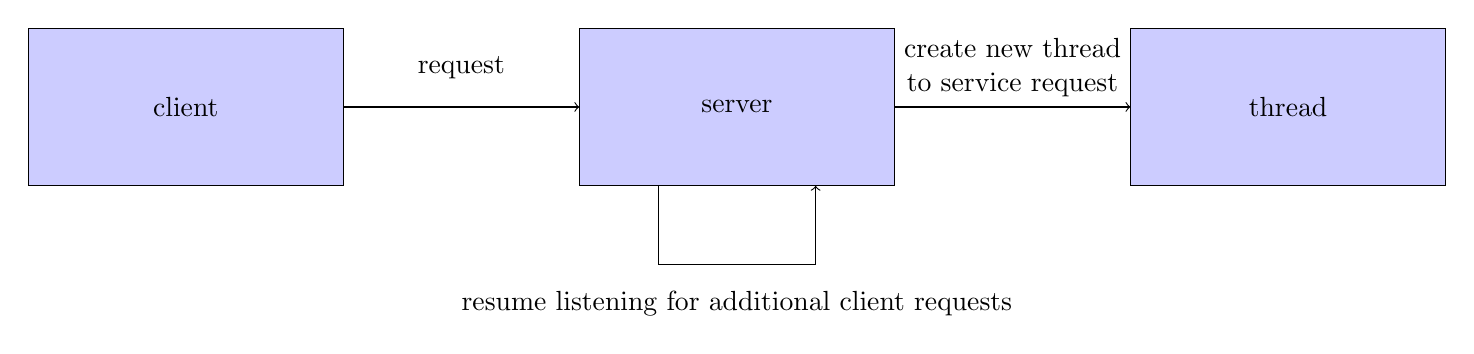
\begin{tikzpicture}
        \draw [fill=blue!20] (0,0) rectangle (4,2);
        \draw [->] (4,1) -- (7,1);
        \draw [fill=blue!20] (7,0) rectangle (11, 2);
        \draw [->] (11,1) -- (14,1);
        \draw [fill=blue!20] (14,0) rectangle (18, 2);
        \draw [->] (8,0) -- (8,-1) -- (10,-1) -- (10,0);
        \node [align=center] at (2,1) {client};
        \node [align=center] at (9,1) {server};
        \node [align=center] at (16,1) {thread};
        \node [align=center] at (5.5, 1.5) {request};
        \node [align=center] at (12.5, 1.5) {create new thread\\to service request};
        \node [align=center] at (9, -1.5) {resume listening for additional client requests};
    \end{tikzpicture}
\end{document}